\documentclass[tikz,border=2pt]{standalone}
\usepackage{amsmath}
\usetikzlibrary{arrows.meta}
\begin{document}
% Jobs at the server L_s^B(t) while one batch of B_k=3 jobs is served, services 20, 30, 25 min:
% heights 3, 2, 1, area Z_k = 3*20 + 2*30 + 1*25 = 145 job-minutes;
% conditional mean B(B+1)/2 E[S] = 6*25 = 150 for E[S]=25 min.
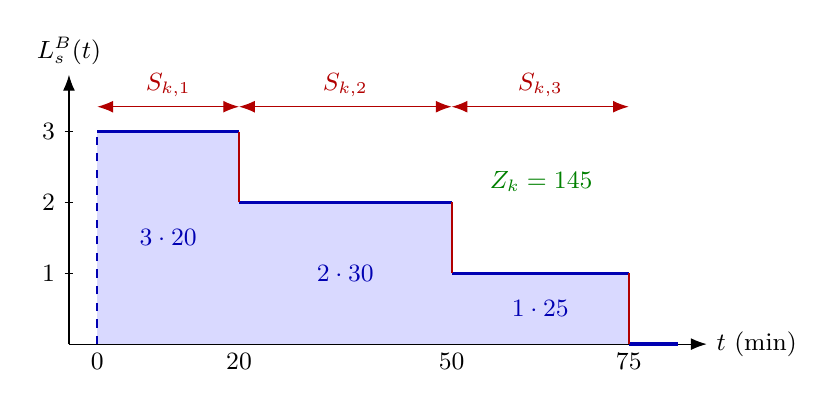
\begin{tikzpicture}[font=\small, >={Latex[length=2mm]}, x=0.09cm, y=0.9cm]
  \fill[blue!15] (0,0) rectangle (20,3);
  \fill[blue!15] (20,0) rectangle (50,2);
  \fill[blue!15] (50,0) rectangle (75,1);
  \draw[->] (-4,0) -- (86,0) node[right] {$t$ (min)};
  \draw[->] (-4,0) -- (-4,3.8) node[above] {$L_s^B(t)$};
  \foreach \y in {1,2,3} \draw (-4.6,\y) -- (-3.4,\y) node[pos=0, left] {$\y$};
  \draw[blue!70!black, very thick] (0,3) -- (20,3) (20,2) -- (50,2) (50,1) -- (75,1) (75,0) -- (82,0);
  \draw[red!70!black, thick] (20,3) -- (20,2) (50,2) -- (50,1) (75,1) -- (75,0);
  \draw[blue!70!black, thick, dashed] (0,0) -- (0,3);
  \node[blue!70!black] at (10,1.5) {$3\cdot20$};
  \node[blue!70!black] at (35,1.0) {$2\cdot30$};
  \node[blue!70!black] at (62.5,0.5) {$1\cdot25$};
  \foreach \x in {0,20,50,75} \node[below] at (\x,0) {$\x$};
  % service-time braces
  \draw[<->, red!70!black] (0,3.35) -- (20,3.35) node[midway, above] {$S_{k,1}$};
  \draw[<->, red!70!black] (20,3.35) -- (50,3.35) node[midway, above] {$S_{k,2}$};
  \draw[<->, red!70!black] (50,3.35) -- (75,3.35) node[midway, above] {$S_{k,3}$};
  \node[green!50!black, anchor=west] at (54,2.3) {$Z_k=145$};
\end{tikzpicture}
\end{document}
